% Zmodyfikowane style z dodaną czcionką \large
\tikzstyle{startstop} = [rectangle, rounded corners, minimum width=3cm, minimum height=1cm, text centered, line width=2pt, draw={rgb,255:red,116; green,39; blue,116}, fill={rgb,255:red,234; green,223; blue,234}]

\tikzstyle{processExcel} = [rectangle, minimum width=3cm, minimum height=1cm, text centered, line width=2pt, draw={rgb,255:red,16; green,124; blue,65}, fill=ForestGreen!80]

\tikzstyle{Variable} = [rectangle, minimum width=3cm, minimum height=1cm, text centered, line width=2pt, draw={rgb,255:red,119; green,11; blue,214}, fill={rgb,255:red,171; green,104; blue,230}]

\tikzstyle{Data} = [rectangle, minimum width=3cm, minimum height=1cm, text centered, line width=2pt, draw={rgb,255:red,140; green,108; blue,255}, fill={rgb,255:red,166; green,141; blue,255}]

\tikzstyle{SP} = [rectangle, minimum width=3cm, minimum height=1cm, text centered, line width=2pt, draw={rgb,255:red,3 ; green,108; blue,112}, fill={rgb,255:red,39; green,181; blue,194}, align=center]

\tikzstyle{decision} = [diamond, minimum width=3cm, minimum height=1cm, text centered, draw=black, fill=green!30]

\tikzstyle{decision} = [diamond, minimum width=3cm, minimum height=1cm, text centered, draw=black, fill=green!30]
\tikzstyle{arrow} = [thick,->,>=stealth]
\tikzstyle{data} = [parallelogram, minimum width=3cm, minimum height=1cm, text centered, draw=black, fill=yellow!30]

\resizebox{0.9\textwidth}{!}{%
\begin{tikzpicture}[node distance=3cm]
   
% Start node
\node (start) [startstop, text width=8cm, align=center] {\textbf{Trigger: Power Apps} \\[4pt]
\begin{tabular}{@{}cc@{}}
    FileName (string) & Year (number) \\
    IndicationNo (number) & Overwrite (bool) \\
\end{tabular}};

% Process nodes
\node (getTables) [processExcel, below of=start, fill=ForestGreen!80, text width=6cm, align=center, yshift=0.5cm] {\textbf{Get Tables} \\[4pt]
(from Excel with name \textit{FileName})};

\node (initializeVars) [Variable, align=center, text width=12cm, below of=getTables, yshift=-0.5cm] {
\textbf{Initialize Variables:}\\[4pt]
\begin{tabular}{@{}ll@{}}
- Excel Table (string) & - ItemsAddedToListaUslug (string) \\
- ItemsAddedToListaKwot (string) & - ItemsAddedToListaIndykacji (string) \\
- BatchRequestHeader (string) & - EndOfBatchRequest (string) \\
- Errors (string) \\
\end{tabular}
};


% Loop
% Twój niestandardowy bloczek jako węzeł
\node (applyToEach) [draw=none, inner sep=0pt, below of=initializeVars, below of=initializeVars, yshift=1.5cm] {%
    \begin{tikzpicture}[baseline]
        \draw [fill={rgb,255:red,152; green,171; blue,193}, draw={rgb,255:red,72; green,105; blue,145}, line width=2pt, dashed] (0,0) rectangle (5.5,-3.5);
        \draw [Variable, text width=4.5cm] (0.25,-1.5) rectangle node {\normalsize \textbf{Set Variable} \\[4pt]
        ExcelFile = TableContent} (5.25,-2.75);
        \node [font=\normalsize] at (2.75,-0.5) {\textbf{Apply to each}};
        \draw [processExcel] (0.25,-0.75) rectangle node {\normalsize \textbf{List rows present in table}} (5.25,-1.5);
    \end{tikzpicture}
};

% Select Columns
\node (selectCols) [Data, below of=applyToEach, text width=6cm, align=center] {\textbf{Select Columns from Excel}};

\node (Condition1) [rectangle, minimum width=3cm, minimum height=1cm, text centered, line width=2pt, draw={rgb,255:red,72; green,79; blue,88}, fill={rgb,255:red,149; green,153; blue,158},below of=selectCols, yshift=1cm, text width = 4cm] {\textbf{Condition 1}\\[4pt] \textit{Overwrite} == false};

\coordinate (belowCondition1) at ($(Condition1.south) - (0,2cm)$);


\node (ComplexNode) [draw=none, inner sep=0pt, anchor=north] at (Condition1.south) {%
    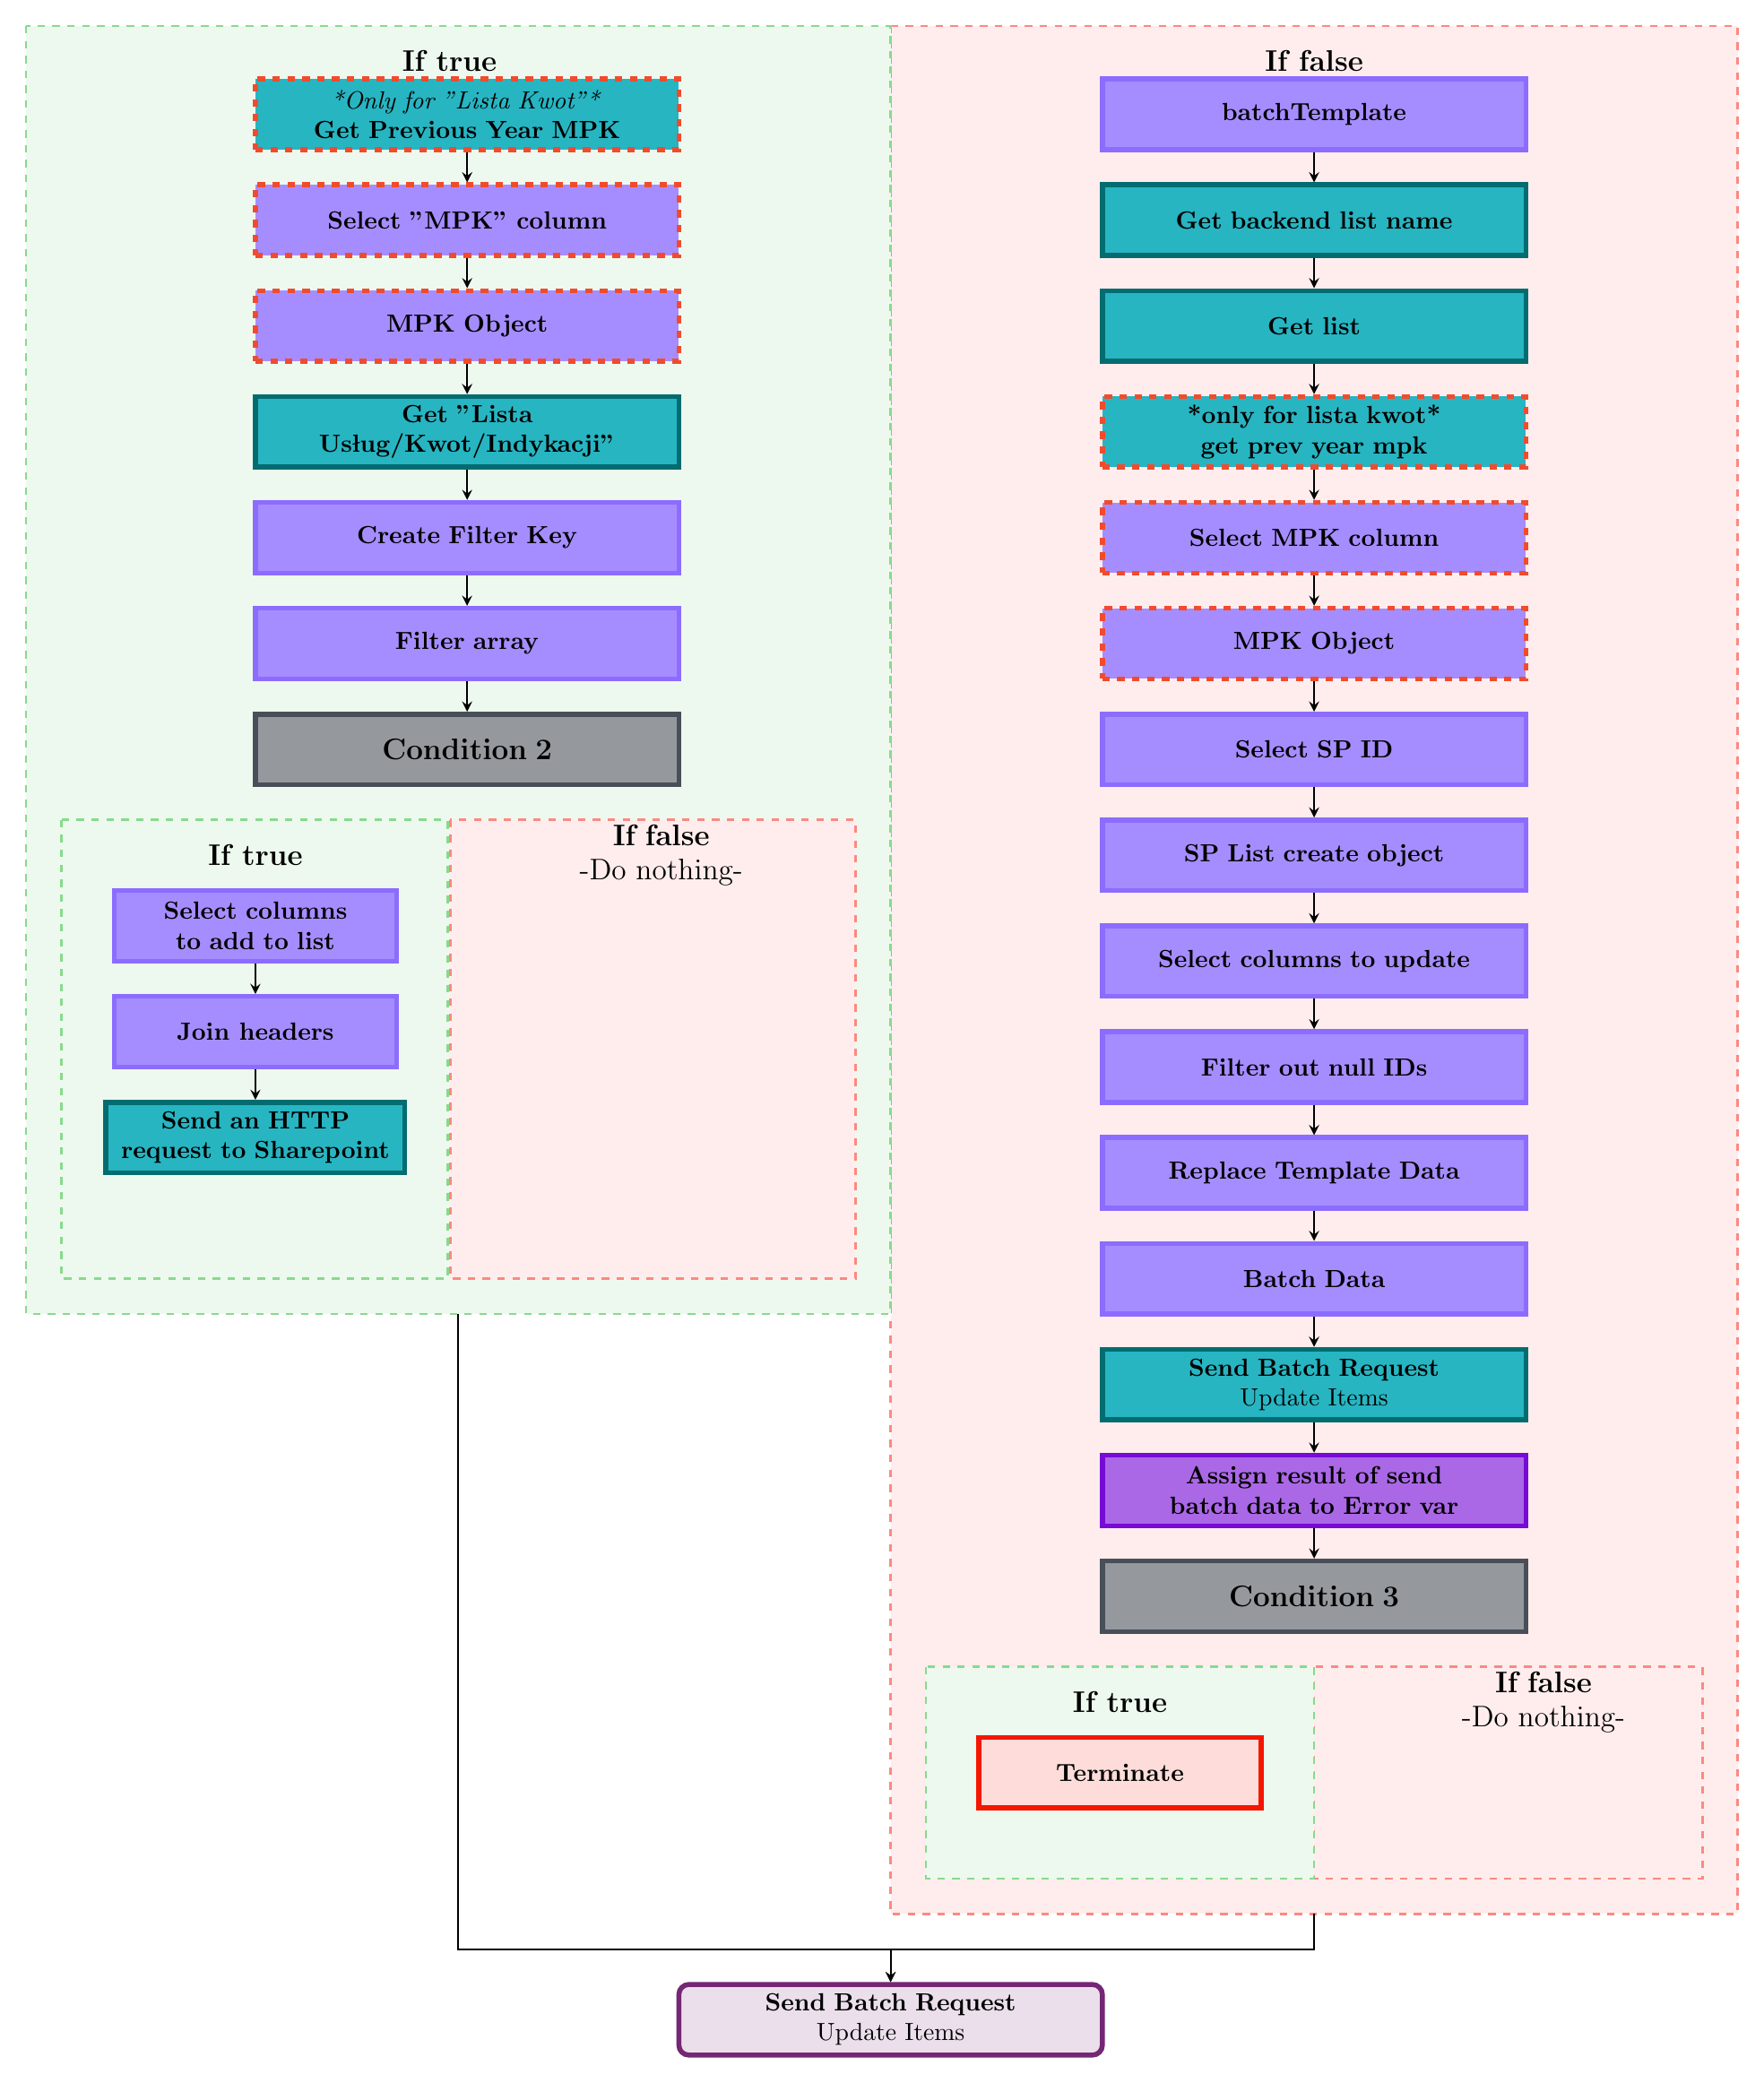
\begin{tikzpicture}[baseline]
\draw [ color={rgb,255:red,251; green,137; blue,129} , fill={rgb,255:red,254; green,237; blue,236}, line width=1pt , dashed] (2,23.75) rectangle  node {}  (14,-3); %false
\draw [ color={rgb,255:red,136; green,218; blue,141} , fill={rgb,255:red,237; green,249; blue,238}, line width=1pt , dashed] (-10.25,23.75) rectangle  node {}  (2,5.5); %true
\node (true1) [SP, dashed, minimum width=6cm, text width=5cm, draw=RedOrange] at (-4,22.5) {\normalsize \emph{*Only for "Lista Kwot"*}\\ \textbf{Get Previous Year MPK}};
\node (true2) [Data, minimum width=6cm, text width=5cm,dashed, draw=RedOrange] at (-4,21) {\normalsize \textbf{Select "MPK" column}};
\node (true3) [Data, minimum width=6cm, text width=5cm,dashed, draw=RedOrange] at (-4,19.5) {\normalsize \textbf{MPK Object}};
\node (true4) [SP, minimum width=6cm, text width=5cm, text width=5cm] at (-4,18) {\normalsize \textbf{Get "Lista Usług/Kwot/Indykacji"}};
\node (true5) [Data, minimum width=6cm, text width=5cm] at (-4,16.5) {\normalsize \textbf{Create Filter Key}};
\node (true6) [Data, minimum width=6cm, text width=5cm] at (-4,15) {\normalsize \textbf{Filter array}};

\draw [ color={rgb,255:red,136; green,218; blue,141} , fill={rgb,255:red,237; green,249; blue,238}, line width=1pt , dashed] (-9.75,12.5) rectangle  node {}  (-4.28,6);
\node (true11) [Data, minimum width=4cm, text width=3cm] at (-7,11) {\normalsize \textbf{Select columns to add to list}};
\node  (true12) [Data, minimum width=4cm] at (-7,9.5) {\normalsize \textbf{Join headers}};
\node  (true13) [SP, minimum width=4cm, text width=4cm] at (-7,8) {\normalsize \textbf{Send an HTTP request to Sharepoint}};
\draw [ color={rgb,255:red,251; green,137; blue,129} , fill={rgb,255:red,254; green,237; blue,236}, line width=1pt , dashed] (-4.24,12.5) rectangle  node {}  (1.5,6);
\node (Condition2) [rectangle, minimum width=3cm, minimum height=1cm, text centered, line width=2pt, draw={rgb,255:red,72; green,79; blue,88}, fill={rgb,255:red,149; green,153; blue,158}, minimum width=6cm, text width=5cm] at (-4,13.5) {\large \textbf{Condition 2}};
\node [font=\large] at (-4.25,23.25) {\textbf{If true}};
\node [font=\large] at (8,23.25) {\textbf{If false}};
\node [font=\large] at (-7,12) {\textbf{If true}};
\node [font=\large, text width=4cm, align=center] at (-1.25,12) {\textbf{If false}\\-Do nothing-};



\node (false1) [Data, minimum width=6cm, text width=5cm] at (8,22.5) { \textbf{batchTemplate}};
\node (false2) [SP, minimum width=6cm, text width=5cm] at (8,21) { \textbf{Get backend list name}};
\node (false3) [SP, minimum width=6cm, text width=5cm] at (8,19.5) { \textbf{Get list}};
\node (false4) [SP, minimum width=6cm, text width=5cm,dashed, draw=RedOrange] at (8,18) { \textbf{*only for lista kwot* \\ get prev year mpk}};
\node (false5) [Data, minimum width=6cm, text width=5cm,dashed, draw=RedOrange] at (8,16.5) { \textbf{Select MPK column}};
\node (false6) [Data, minimum width=6cm, text width=5cm,dashed, draw=RedOrange] at (8,15) { \textbf{MPK Object}};
\node (false7) [Data, minimum width=6cm, text width=5cm] at (8,13.5) {\textbf{Select SP ID}};
\node (false8) [Data, minimum width=6cm, text width=5cm] at (8,12) { \textbf{SP List create object}};
\node (false9) [Data, minimum width=6cm, text width=5cm] at (8,10.5) { \textbf{Select columns to update}};
\node (false10) [Data, minimum width=6cm, text width=5cm] at (8,9) { \textbf{Filter out null IDs}};
\node (false11) [Data, minimum width=6cm, text width=5cm] at (8,7.5) { \textbf{Replace Template Data}};
\node (false12) [Data, minimum width=6cm, text width=5cm] at (8,6) { \textbf{Batch Data}};
\node (false13) [SP, minimum width=6cm, text width=5cm] at (8,4.5) { \textbf{Send Batch Request}\\ Update Items};
\node (false14) [Variable, minimum width=6cm, text width=5cm] at (8,3) { \textbf{Assign result of send batch data to Error var}};

\draw [ color={rgb,255:red,251; green,137; blue,129} , fill={rgb,255:red,254; green,237; blue,236}, line width=1pt , dashed] (8,0.5) rectangle  node {}  (13.5,-2.5);
\draw [ color={rgb,255:red,136; green,218; blue,141} , fill={rgb,255:red,237; green,249; blue,238}, line width=1pt , dashed] (2.5,0.5) rectangle  node {}  (8,-2.5);
\node[Data, minimum width=4cm, draw={rgb,255:red,244; green,23; blue,0} , fill={rgb,255:red,253; green,220; blue,217}] at (5.25,-1) {\normalsize \textbf{Terminate}};
\node (Condition3) [rectangle, minimum width=3cm, minimum height=1cm, text centered, line width=2pt, draw={rgb,255:red,72; green,79; blue,88}, fill={rgb,255:red,149; green,153; blue,158}, minimum width=6cm, text width=5cm] at (8,1.5) {\large \textbf{Condition 3}};
    \node [font=\large] at (5.25,0) {\textbf{If true}};
\node [font=\large, text width=4cm, align=center] at (11.25,0) {\textbf{If false}\\-Do nothing-};

\node (stop) [startstop, minimum width=6cm, text width=5cm] at (2,-4.5) { \textbf{Send Batch Request}\\ Update Items};

%Arrows
\draw [arrow] (true1) -- (true2);
\draw [arrow] (true2) -- (true3);
\draw [arrow] (true3) -- (true4);
\draw [arrow] (true4) -- (true5);
\draw [arrow] (true5) -- (true6);
\draw [arrow] (true6) -- (Condition2);

\draw [arrow] (true11) -- (true12);
\draw [arrow] (true12) -- (true13);

\draw [arrow] (false1) -- (false2);
\draw [arrow] (false2) -- (false3);
\draw [arrow] (false3) -- (false4);
\draw [arrow] (false4) -- (false5);
\draw [arrow] (false5) -- (false6);
\draw [arrow] (false6) -- (false7);
\draw [arrow] (false7) -- (false8);
\draw [arrow] (false8) -- (false9);
\draw [arrow] (false9) -- (false10);
\draw [arrow] (false10) -- (false11);
\draw [arrow] (false11) -- (false12);
\draw [arrow] (false12) -- (false13);
\draw [arrow] (false13) -- (false14);
\draw [arrow] (false14) -- (Condition3);


\draw [arrow] (-4.125,5.5) -- +(0,-9) -- +(6.125,-9) --(stop);
\draw [arrow] (8,-3) -- +(0,-0.5) -- +(-6,-0.5) --(stop);

\end{tikzpicture}

};
\draw [arrow] (start) -- (getTables);
\draw [arrow] (getTables) -- (initializeVars);
\draw [arrow] (initializeVars) -- (applyToEach);
\draw [arrow] (applyToEach) -- (selectCols);
\draw [arrow] (selectCols) -- (Condition1);
\draw [arrow] (Condition1) -- (ComplexNode);

\end{tikzpicture}
}